\section{Data}\label{sec:data}


\subsection{Datasets for self-supervised audio modeling}
We use the TIMIT dataset for learning audio models using stacked WaveNets. 
The TIMIT dataset contains 5.4 hours of audio sampled at 16 kHz, consists of 630 speakers speaking ten sentences, and is a benchmark for Automatic Speech Recognition system \cite{garofolo_john_s_timit_1993}.
Assuming a phoneme rate of $\approx 150/\mathrm{min}$, the TIMIT dataset contains approximately 500K tokens.
% It is therefore small enough for an audio model as the WaveNet to reach convergence relatively quickly. 


The Librispeech dataset contains 960 hours of audio from the public-domain LibriVox audiobooks \cite{noauthor_librispeech_nodate}.
LibriSpeech contains two "clean" splits, \texttt{clean\_100} and \texttt{clean\_360}, as well as a non-clean, \texttt{other\_500} split. 
The corresponding Libri-light dataset contains over 60 000 hours of raw audio data, with a 10-hour subset of Librispeech as its labeled \texttt{train} set. 
We use the Librilight dataset as a benchmark for ASR to evaluate and compare pre-trained models trained unsupervised on Librispeech.

% The TIMIT corpus was manually designed for ASR experiments it's phonetically rich and varied dialectically in spite of its relatively small size - the full LibriSpeech dataset, by contrast, has 960 hours of audiobook audio. 

\subsection{Modality and transformation of data}\label{ssec:data-modality}

The original WaveNet papers theorize that the receptive field limits the architecture from modeling full semantic content, partially due to the high sample rate used in audio datasets \cite{oord_wavenet_2016}.
When working with high sample rates, other authors using WaveNet architectures have reported success by increasing the convolution filter size from 2 to 3 \cite{oord_parallel_2017}.
The authors of the Parallel WaveNet further suggest that adding more dilation stages or adding more layers to increase the receptive field of the WaveNet \cite{oord_parallel_2017}.
On the other hand, some probabilistic generative models for sequence modeling %, like the SRNN and VRNN,
predict $S$-frame stacked vectors of audio waveforms \cite{fraccaro_sequential_2016, chung_recurrent_2016}.
This is equivalent to transforming $\mathbf{x}$ as below:
\begin{equation}\label{data:eq-transform}
    % \mathbf{x}\in \mathbb{R}^N \hspace{0.5cm} x_t \in \mathbb{R} \rightarrow \mathbf{x}^*\in \mathbb{R}^{N/S, S}, \hspace{0.5cm} x_t \in \mathbb{R}^S \\
    % \mathbf{x}^* = \begin{pmatrix}
    %     x_1 & x_{S+1} & \dots & x_{N-S} \\
    %     \vdots & \vdots &  & \vdots \\
    %     x_{S} & x_{2S} & \dots & x_N
    % \end{pmatrix}, \quad 
    \mathbf{x}^*_t = \begin{pmatrix}
        x_{t} \\ \vdots \\ x_{t+S} \\
    \end{pmatrix},
\end{equation}
for $t\in\{1,S+1,\dots,T-S\}$ and $\mathbf{x}^*\in\mathbb{R}^{N/S \times S}$ and $\mathbf{x}\in\mathbb{R}^{N}$.

While these models reach state-of-the-art log-likelihoods for on-step prediction, the method has met criticism for allowing models to leak a subset of $x_t$ through the latent variable $z_t$ \cite{dai_re-examination_2019}. 
By optimizing an output distribution 
\[
p_\theta(x_t | \mathbf{x}) \approx \prod_{i=1}^L p_\theta (x_{t,i}|\mathbf{z}_{\leq t} , \mathbf{x}_{<t}) \enspace ,
\]
the learnt posterior $q(z_t|x_t)$ allows for conditioning on $x_t$.
Thus the model can interpolate the remaining steps using the intra-step correlation in the output vector and artificially increase performance. \cite{dai_re-examination_2019}
This problem does not arise in the WaveNet architecture, as the causal architecture of the model ensures that the model predicts next-step, not on-step. 

\subsubsection{Mu-law encoding}
$\mu$-law encoding is a signal-processing tool used to compress 16 bit PCM to 8-bit logarithmic data.
The encoding is explicitly designed to work with speech, as high-frequency components dominate speech audio signals. \cite{noauthor_-law_2008}

$b$-bit $\mu$-law encoding transforms the input $x$ according to the following equation:
\begin{equation}
    F(x) = \sign(x) * \frac{\ln(1 + \mu |x|)}{\log (1-\mu)}, \hspace{.5cm} \mu = 2^b
\end{equation}
The $\mu$-law encoding is reversible and the decoding transforms outputs as:
\begin{equation}
G(x) = \sign(x)*\frac{\exp(|x|*\log (1-\mu))}{\mu}
\end{equation}

For audio modeling purposes, $\mu$-law encoding allows the model to use a broader spectrum of its output space, as illustrated in \cref{fig:mu-law-enc}.
\cite{oord_wavenet_2016}


\begin{figure}[ht]
    \centering
    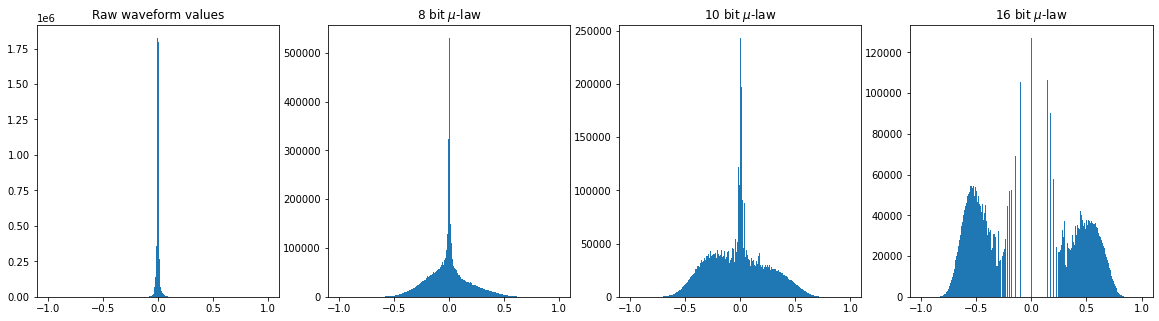
\includegraphics[width=\columnwidth]{mu_law.png}
    \caption{
    Illustration of the distribution of raw PCM values from the TIMIT test set which are natively 16-bit integers and the corresponding distribution after $\mu$-law encoding the waveform values with different values of $\mu$.
    At 16 bits, all areas of the spectrum are covered while not overpopulated at the extreme bins.
    }
    \label{fig:mu-law-enc}
\end{figure}



